\documentclass[12pt]{article}
\usepackage{lmodern}
\usepackage[T1]{fontenc}
\usepackage[dvips,letterpaper,margin=0.75in,bottom=0.75in]{geometry}
%\usepackage[dvips,letterpaper,margin=1in,bottom=1in]{geometry}
\usepackage{cancel}
\usepackage{graphicx}
\usepackage{braket}
\usepackage{latexsym,amssymb,amsmath}
\usepackage{pdfpages}
\usepackage{xcolor}
\usepackage{capt-of}
\usepackage{amsmath}
\usepackage{cite}
\usepackage{lineno}
\usepackage[hyperfootnotes=false,hidelinks]{hyperref}
\usepackage[shortlabels]{enumitem}
\usepackage{pdfpages}
\newcommand{\tcr}{\textcolor{red}}
\newcommand{\tcb}{\textcolor{blue}}

\usepackage[american,fulldiode]{circuitikz}
\tikzset{component/.style={draw,thick,circle,fill=white,minimum size =0.75cm,inner sep=0pt}}

\begin{document}
\ctikzset{bipoles/thickness=1}
\ctikzset{bipoles/length=.6cm}


%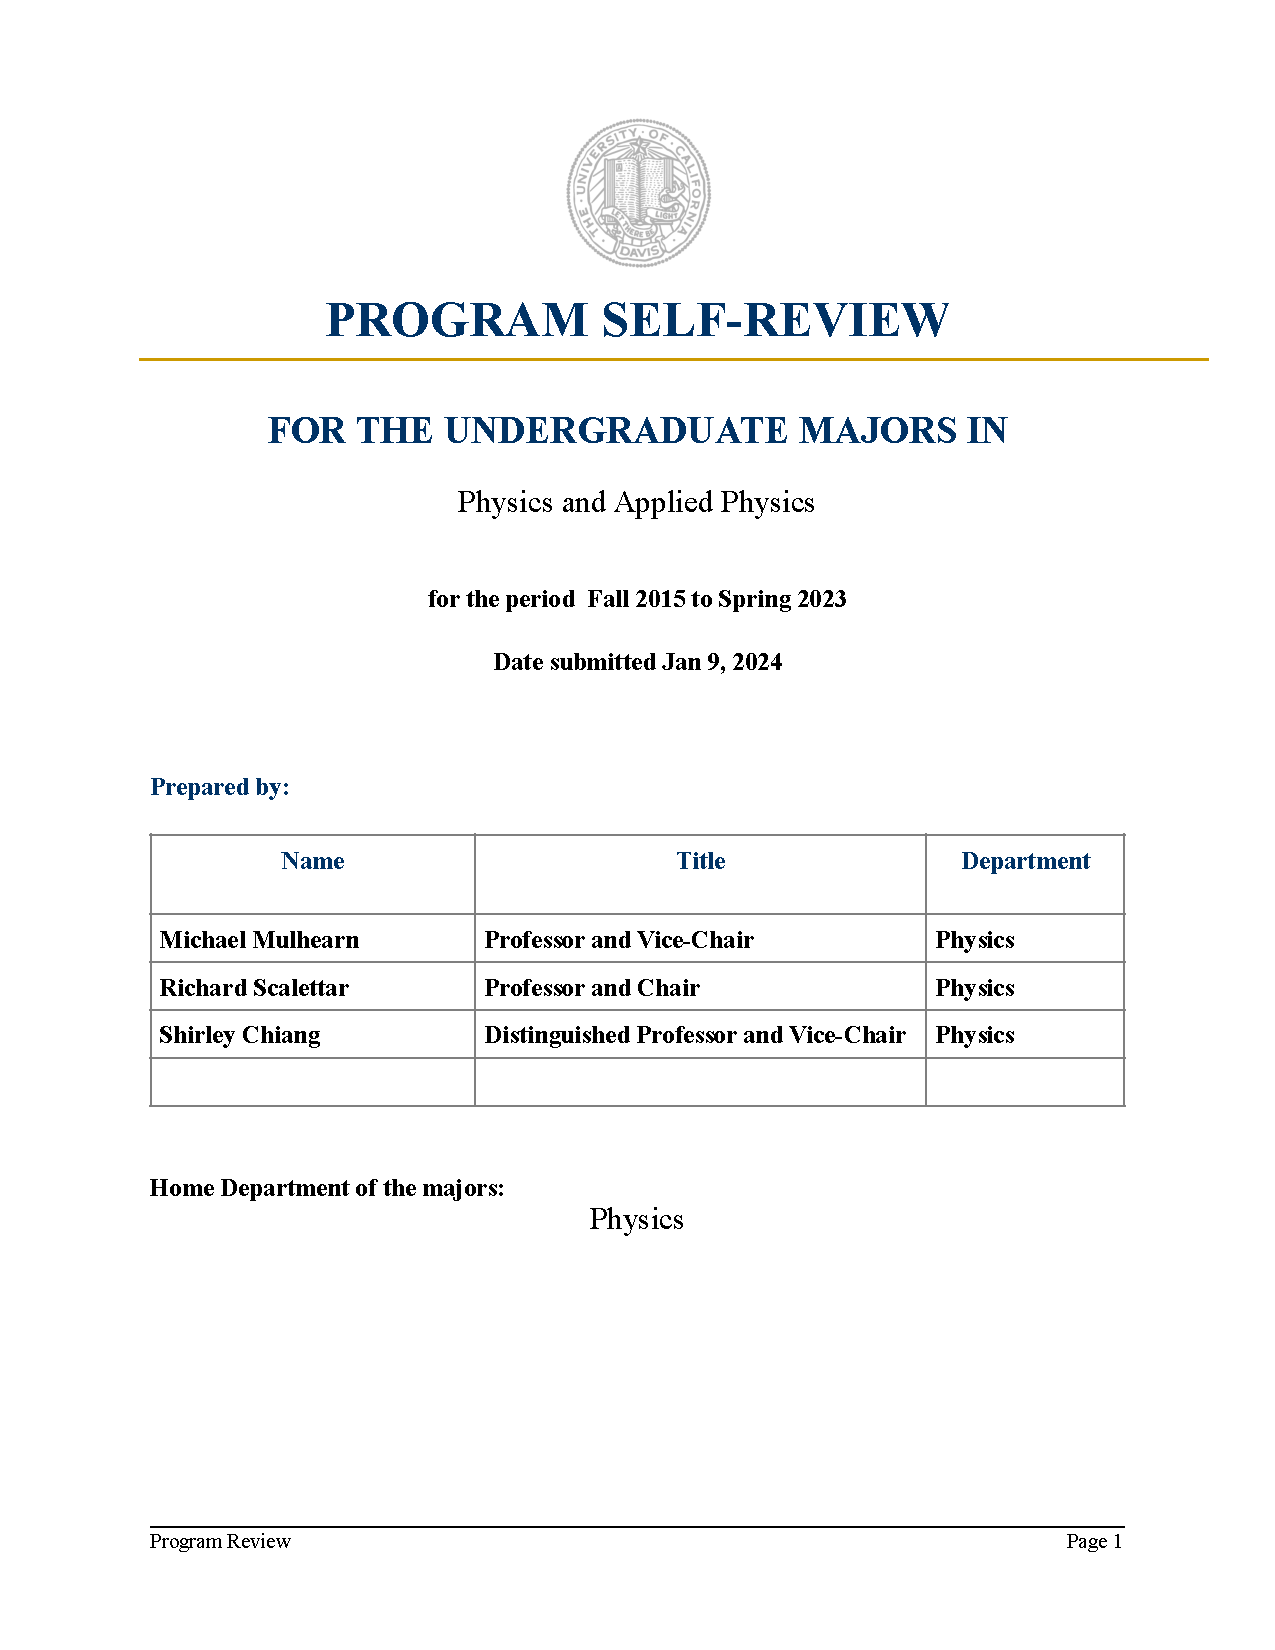
\includepdf[pages=-]{physics_cover.pdf}


\newpage
\section{PHY 122A:  Advanced Lab in Physics -- Writing Experience}

This summary refers to the minimal elements of the Writing
Experience\footnote{
\href{https://ge.ucdavis.edu/sites/g/files/dgvnsk4376/files/inline-files/final\_writing\_experience\_8.20.20.pdf}{https://ge.ucdavis.edu/sites/g/files/dgvnsk4376/files/inline-files/final\_writing\_experience\_8.20.20.pdf (click)}}.  The material submitted for this in-depth review was prepared by Prof. Matthew
Citron\footnote{Citron is nominally assigned to PHY 122B, but the course is team taught.}
from a class he taught in Spring 2023.  PHY 122B (Particle
Physics) and PHY 122A (Condensed Matter Physics) are team taught,
simultaneously, which is why the included course material will refer
to only PHY 122.  All supporting documentation is available in Appendix~\ref{sec:supa}.\\

\noindent
{\bf (ME1) Demonstrate that writing is a central component of the course:}
Students conduct two elective experiments during the course and prepare a lab
report for each one.\\[2pt]

\noindent
{\bf (ME2) Show that students are trained in the writing conventions of the relevant discipline:}\\
See ``Preparting a Report on Your Experiment'' which includes an overview, links to a 25 slide talk, APS style instructions, and example texts. \\[3pt]
\noindent
{\bf (ME3) Assure that model texts are provided and discussed:}\\
Four example scientific articles are provided on the course website.  These are referred to for concrete examples when discussing the writing conventions and other issues that arise.\\[3pt]

\noindent
{\bf (ME4) Demonstrate that the 5/10 page (1500/3000 words) writing assignment(s) requirement is
met. Revisions are encouraged, but revisions of past submissions do not count toward the 10-
page minimum:} Students prepare two reports, each typically 8-16 pages, and always more than 10 pages total.  The course includes revisions, but those have not been counted here.

\noindent
{\bf (ME5) Provide specific demonstration and explanation of the evaluation criteria:}
The rubric used to grade the reports is included in the section on preparing reports.\\[1pt]

\noindent
{\bf ME6) Demonstrate that individual feedback from instructors or teaching assistants is integrated into the course in a manner designed to promote improvement in writing:}
As explained in the course overview, students are given feedback on their first report, which they revise and submit for a final grade.\\[1pt]

\noindent
{\bf (ME7) Show that guidance on plagiarism is provided.}
Plagiarism results in an F for the course.  Three useful resources are provide to explain plagiarism.\\[1pt]

\noindent
{\bf (ME8) Demonstrate that the learning objectives of the literacy are an integral part of the class.}
The lab report is the ultimate deliverable for each of the three experiments conducted during the course.  Students are encouraged to begin drafting their report as soon as they have developed a written plan.\\[1pt]

\section{AST 10G: Intro to  Stars, Galaxies, and the Universe -- Visual Literacy}

This summary refers to the minimal elements of Visual Literacy\footnote{
\href{https://ge.ucdavis.edu/sites/g/files/dgvnsk4376/files/inline-files/final_visual_literacy_0.pdf}{
https://ge.ucdavis.edu/sites/g/files/dgvnsk4376/files/inline-files/final\_visual\_literacy\_0.pdf (click)}}
The material submitted for this in-depth review was prepared by Prof. Andrew
Wetzel from a class he taught in Fall 2023.\\

{\bf (ME1) Identify the type of visual materials or media employed in the class. These
may include still and moving images, art and architecture, illustration
accompanying written text, graphs and charts, or other visual embodiments of
ideas:} From the syllabus:  ``scientific images, movies, figures, charts, and tables''.\\[1pt]

{\bf (ME2) Specify how the course enables students to think critically about visual
  materials:} An example is provided in the course overview:  for example, we will ask you to interpret images and spectra from astronomical objects, including what these can tell us physically about these objects.\\[1pt]

{\bf (ME3) Specify the ways in which students will use or interact with these materials
throughout the course and how frequently they will be used in lectures, student
work and/or examination and assessment:} The example from ME2 applies here, but also from the the course overview:  ``You also will develop skills to interpret x-y type plots, charts, and tables of astronomical data.  We will employ such visual analysis in every class\ldots''\\[1pt]

{\bf (ME4) Identify specific guidelines or metrics for evaluating the students’
understanding of visual literacy (e.g. through examination, written analysis,
production of visual materials, and so on):}
An example of student work from an examination provides a specific
example of students preparting their own visual media (a
Hertzsprung-Russel diagram in this case).  The points assigned to each
part are indicated.  The examples from ME2 and M5 also apply here.

{\bf (ME5) Demonstrate that achieving the minimum set of learning objectives of the
literacy is an integral part of the class:} From the course overview:  ``we will evaluate your understanding through weekly reading quizzes, weekly problem sets, and 3 exams, which will include both intepreting visual data and communicating your answers through visual means.''\\[1pt]

\newpage
\section{AST 10C: Intro to Cosmology -- Scientific Literacy}

This summary refers to the minimal elements of the Scientific Literacy \footnote{
\href{https://ge.ucdavis.edu/sites/g/files/dgvnsk4376/files/inline-files/final_scientific_10.25.19.pdf}{https://ge.ucdavis.edu/sites/g/files/dgvnsk4376/files/inline-files/final\_scientific\_10.25.19.pdf (click)}}
The material submitted for this in-depth review was prepared by Prof. Lori Lubin
from a class she taught in Spring 2023.

You will learn all the clever ways that astrophysicists have come to understand the cosmos so well (despite sitting on some small rock!) -- all the way from posing the relevant scientific questions, determining what observational data to collect, interpreting that data, and finally to developing theories (Hint: It is not "just" a theory!). You will try your own hand at interpreting astronomical images (not just pretty pictures!) and graphs (is that a correlation?) to see how astrophysicists use these critical visual tools to understand our Universe. Finally, science does not progress in a vaccum, so you will learn how cosmology research over the past century was crucially aided by, and contributed to, significant technology and engineering gains (just look at the new James Webb Space Telescope!). 

{\bf (ME1) Demonstrate that a substantial portion of the course covers scientific methods: posing
  questions, gathering data, making conclusions and generating new hypothesis when appropriate:}From the course description:  ``You will learn all the clever ways that astrophysicists have come to understand the cosmos so well (despite sitting on some small rock!) -- all the way from posing the relevant scientific questions, determining what observational data to collect, interpreting that data, and finally to developing theories (Hint: It is not "just" a theory!). You will try your own hand at interpreting astronomical images (not just pretty pictures!) and graphs (is that a correlation?) to see how astrophysicists use these critical visual tools to understand our Universe.''\\[1pt]

{\bf (ME2) Demonstrate that the course covers how scientific findings relate to other disciplines\footnote{Please note that no other literacy includes such an ME, to demonstrate how the discipline targeted by the literacy relates to other disciplines.  Is science of no interest on its own?} and public policy:}From the course description ``Finally, science does not progress in a vaccum, so you will learn how cosmology research over the past century was crucially aided by, and contributed to, significant technology and engineering gains (just look at the new James Webb Space Telescope!).''\\[1pt]

{\bf (ME3) Provide specific demonstration and explanation of the evaluation criteria referring to the
scientific literacy:} The provided assignment has students interpreting scientific results, and then applying scientific methods.  The grading rubric (and its application to example student work) is shown.\\

{\bf (ME4) Demonstrate the achieving the minimum set of learning objectives of the literacy is an
  integral part of the class:}  The overall importance of ME1 and ME2 is stressed in the course overview.  The provided example of student work provides further evidence, in that students are expected to master ME1.\\

\appendix

\newpage
\section{Supporting Material: PHY 122A}
\label{sec:supa}

This section includes the supporting material for PHY 122A.

If you are online, it may be more convenient to peruse the course
website: \href{https://122.physics.ucdavis.edu}{https://122.physics.ucdavis.edu
  (click)}

Actual student work is not included in this appendix and will be
provided separately.  (Even though it is redacted, we prefer to keep
it separate from this report, which is public.)

\newpage
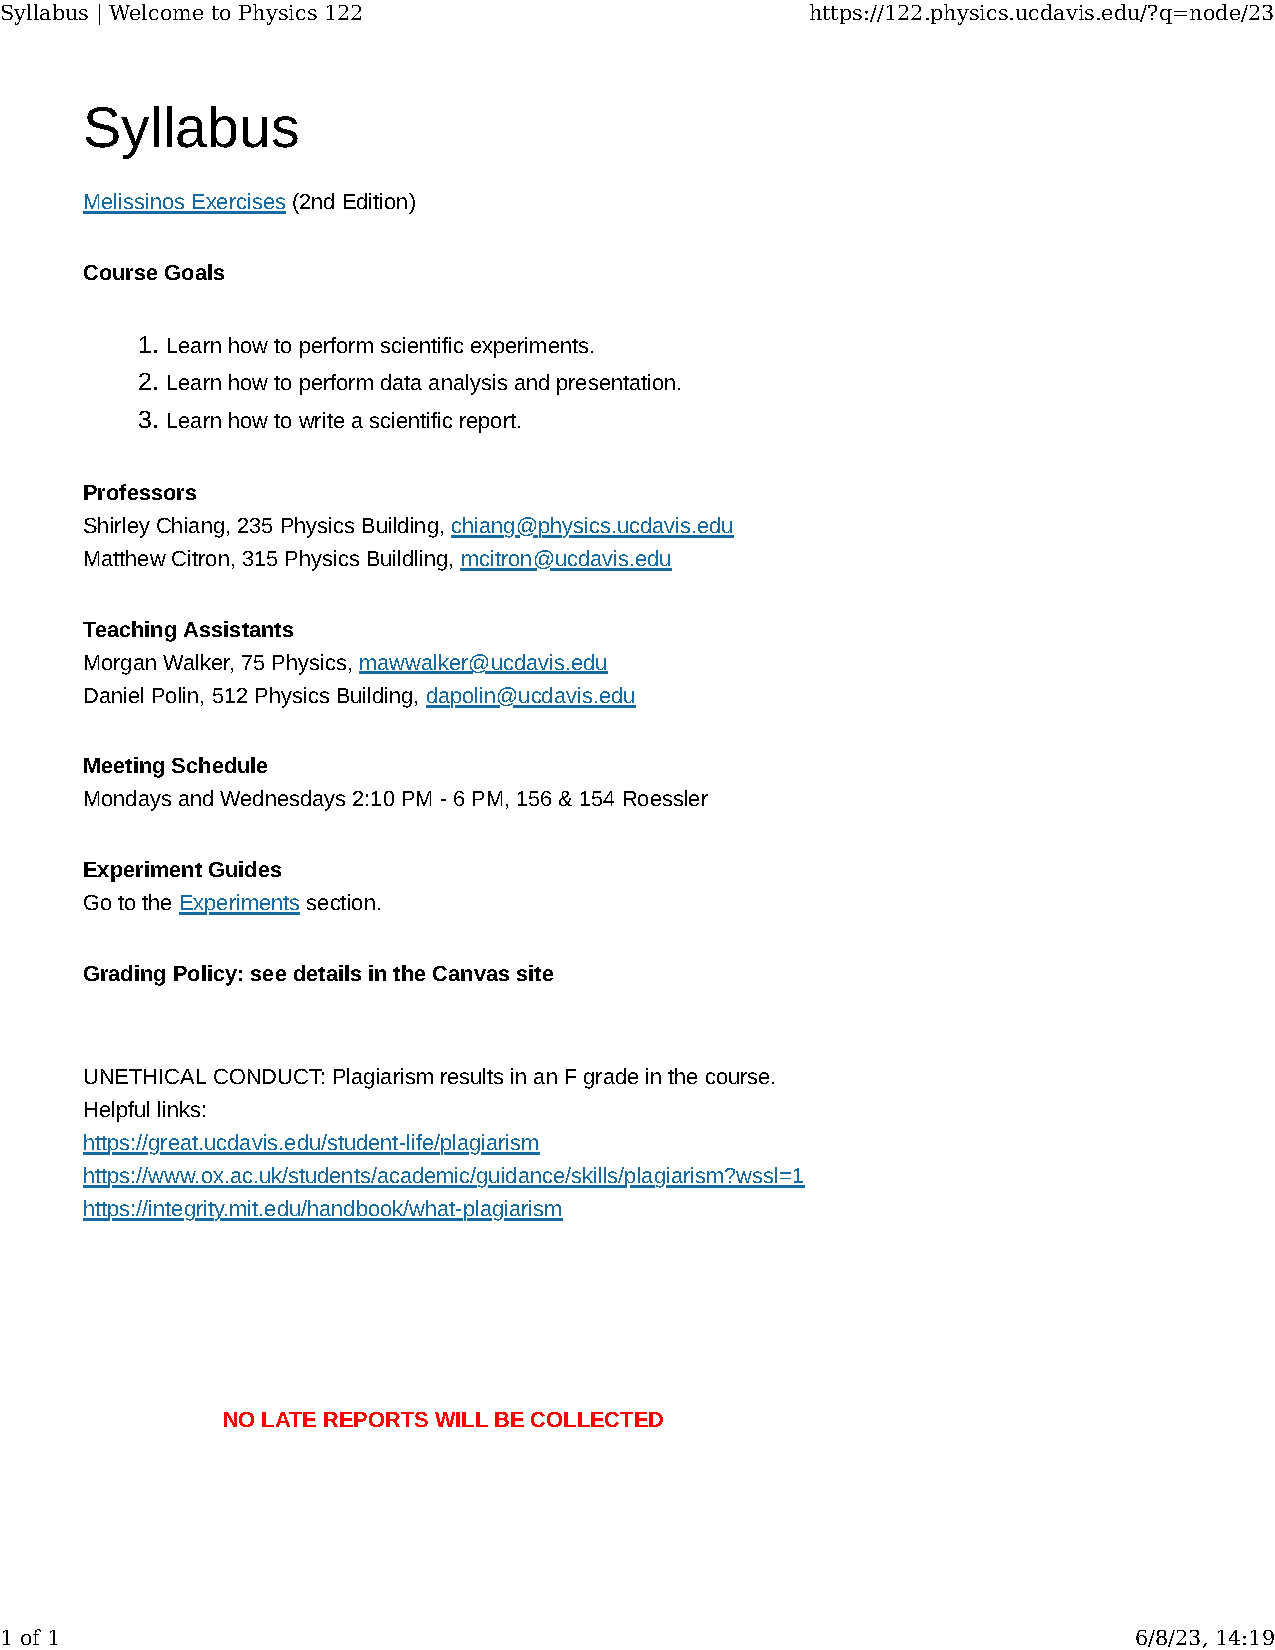
\includepdf[pages=-]{122a/syllabus.pdf}
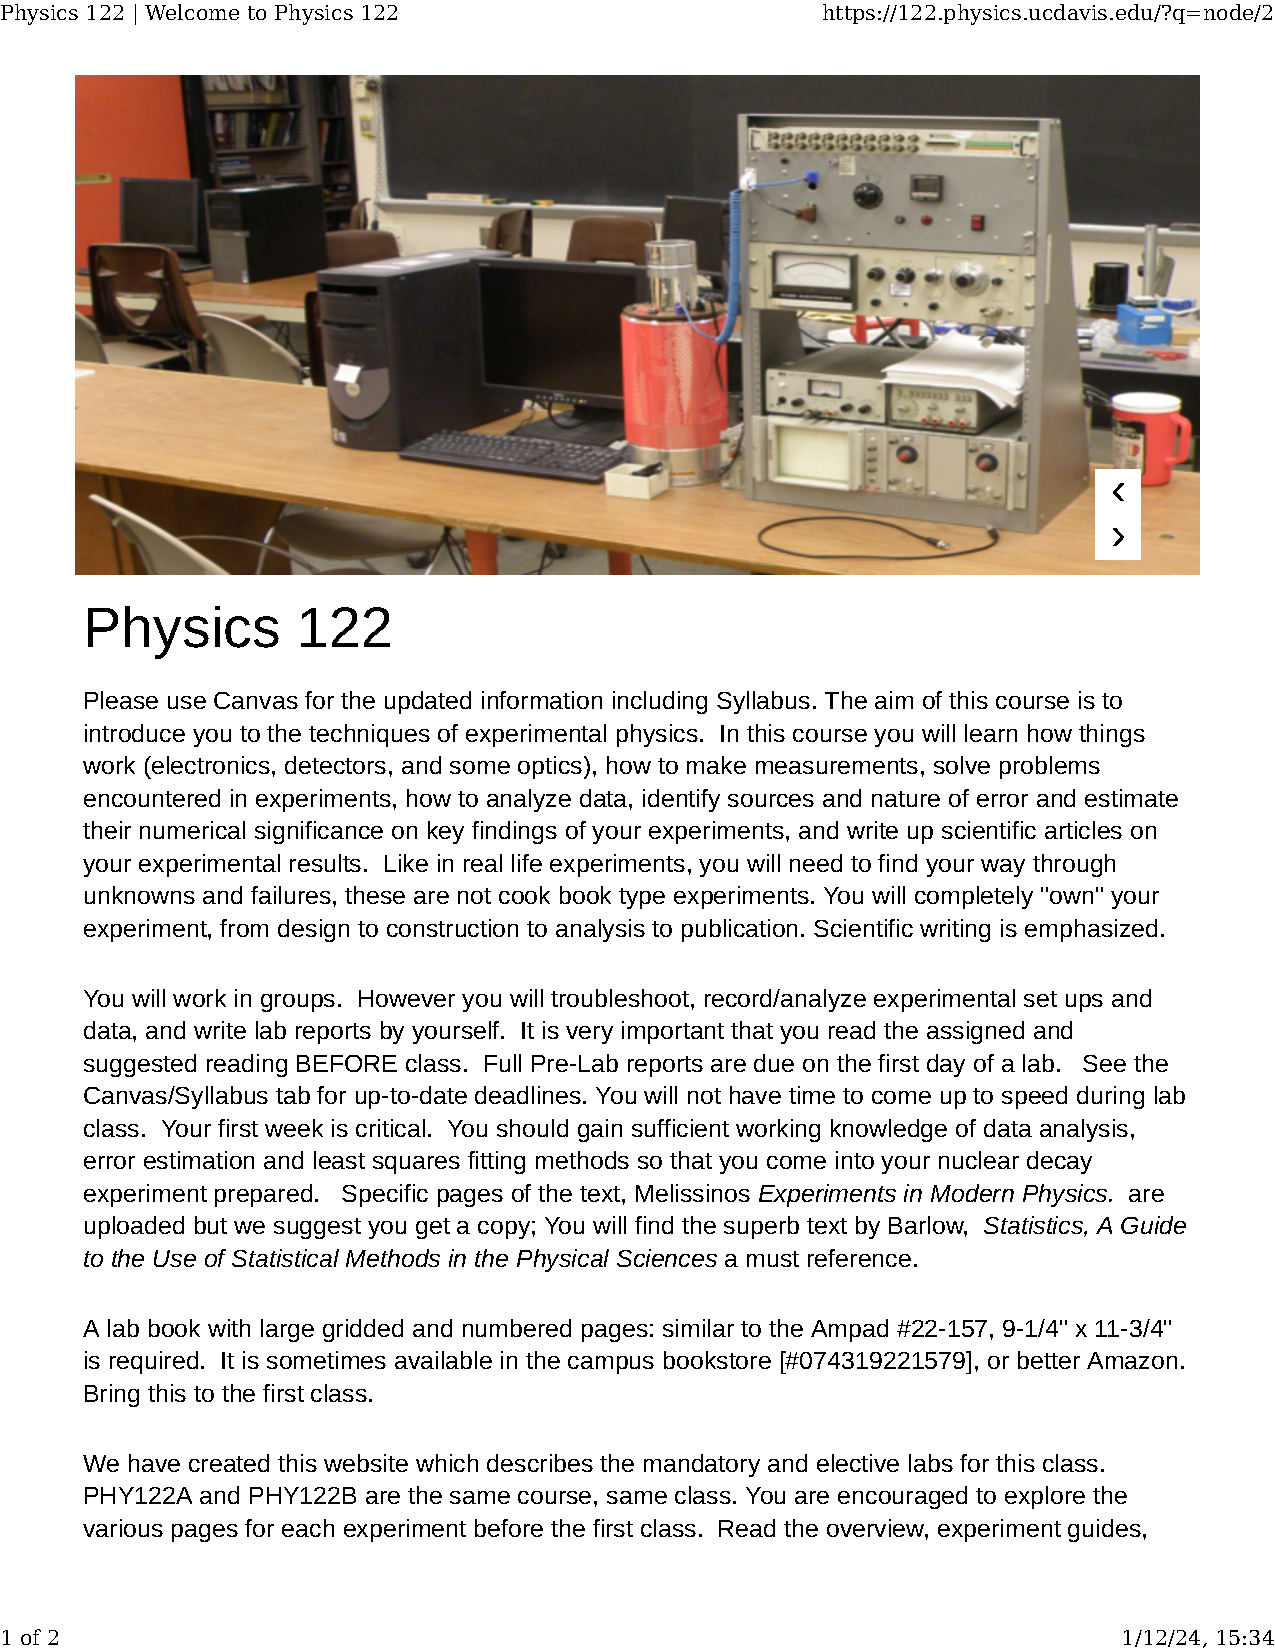
\includepdf[pages=-]{122a/overview.pdf}
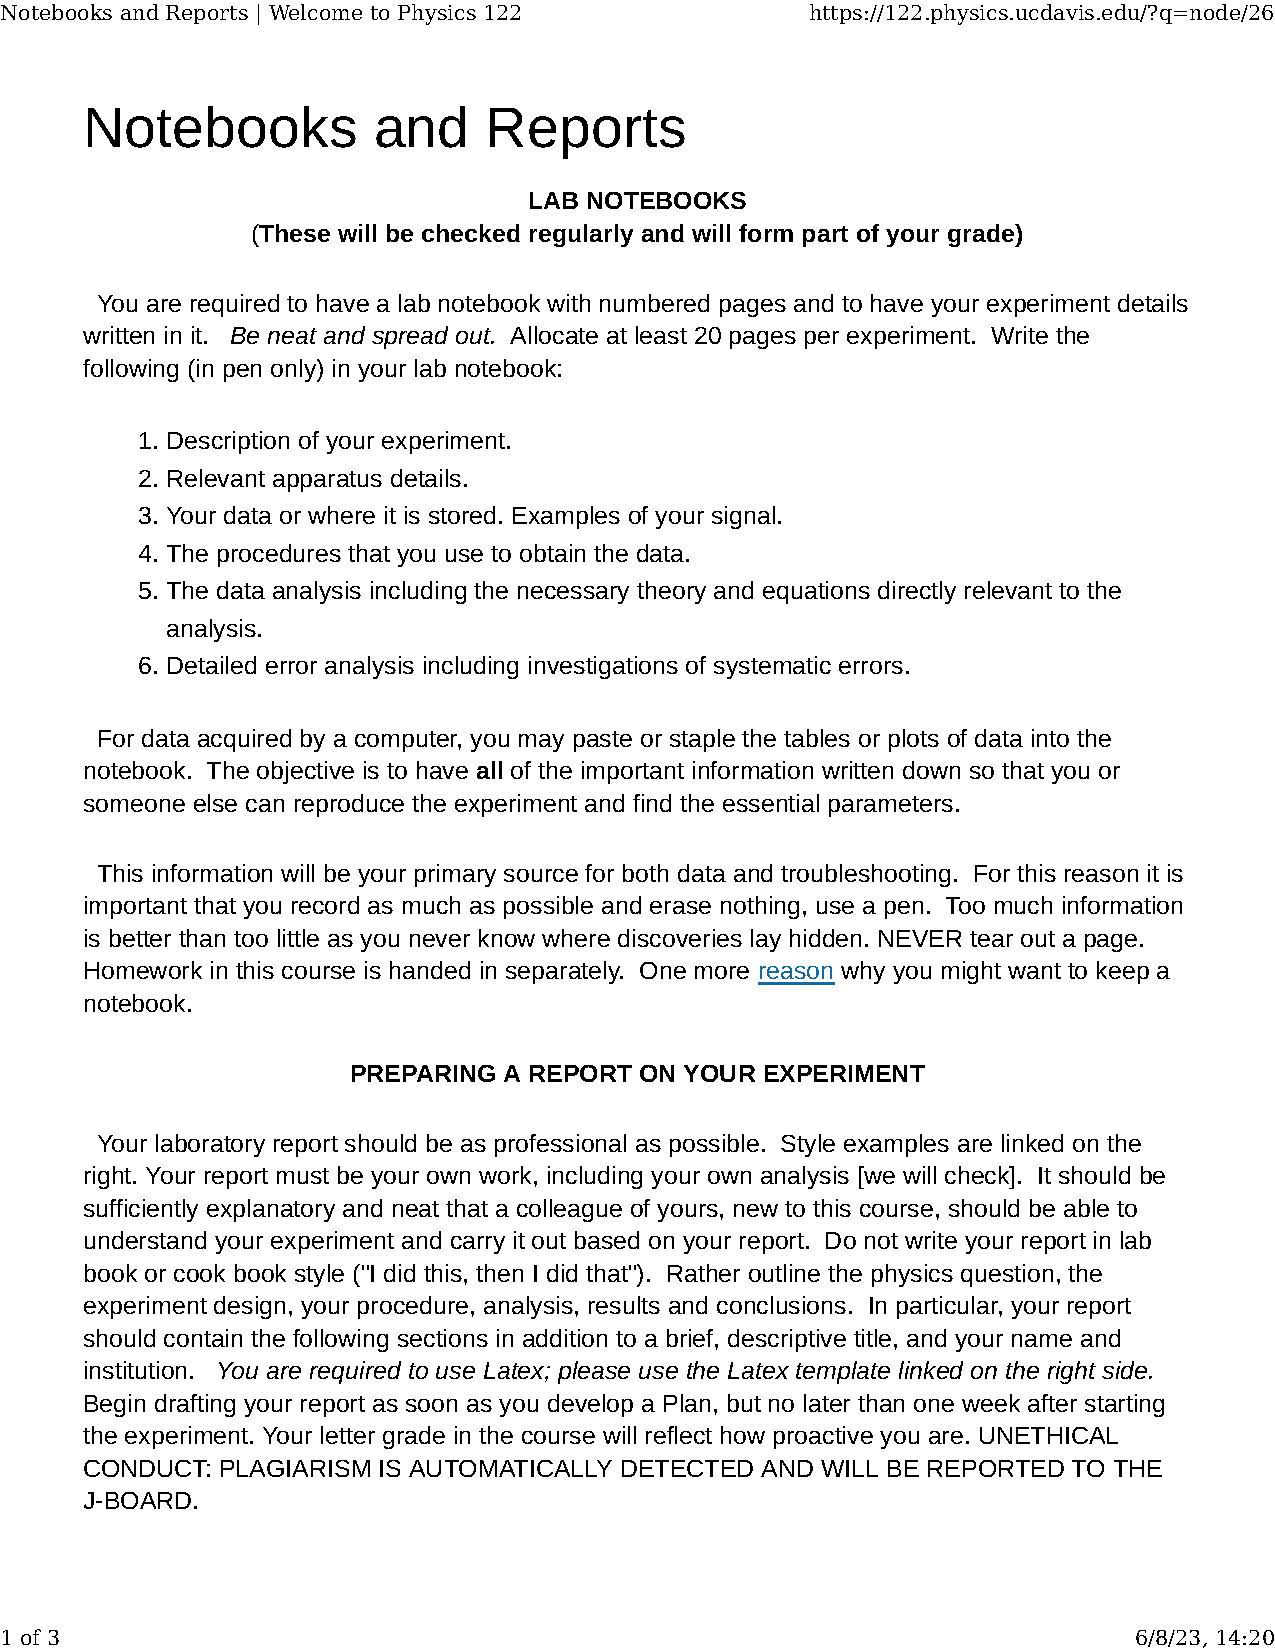
\includepdf[pages=-]{122a/reports.pdf}  


\section{Supporting Material: AST 10G}
\label{sec:supb}
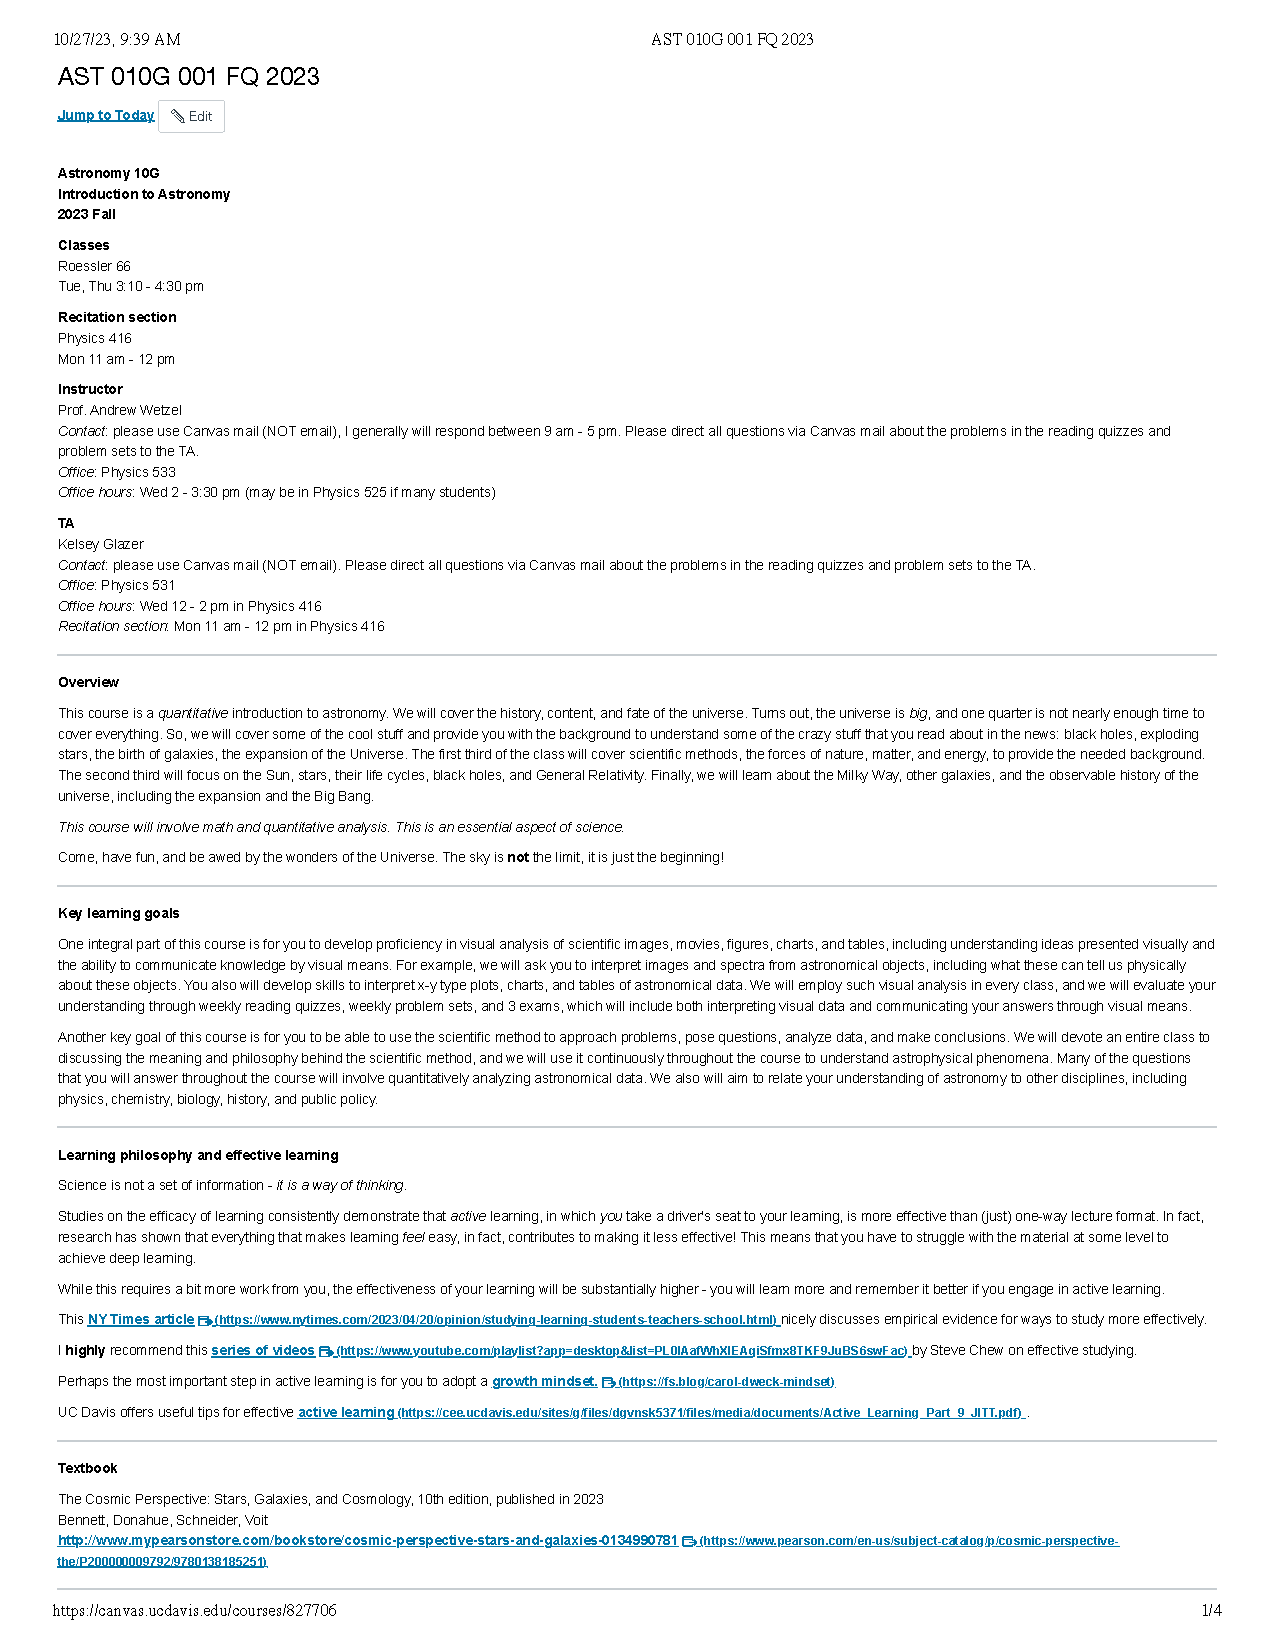
\includepdf[pages=-]{10g/syllabus.pdf}  

\newpage
\section{Supporting Material: AST 10C}
\label{sec:supc}

This section includes the supporting material for AST 10C.

Actual student work is not included in this appendix and will be
provided separately.  (Even though it is redacted, we prefer to keep
it separate from this report, which is public.)  This student work
includes the assignment and rubric.

\newpage

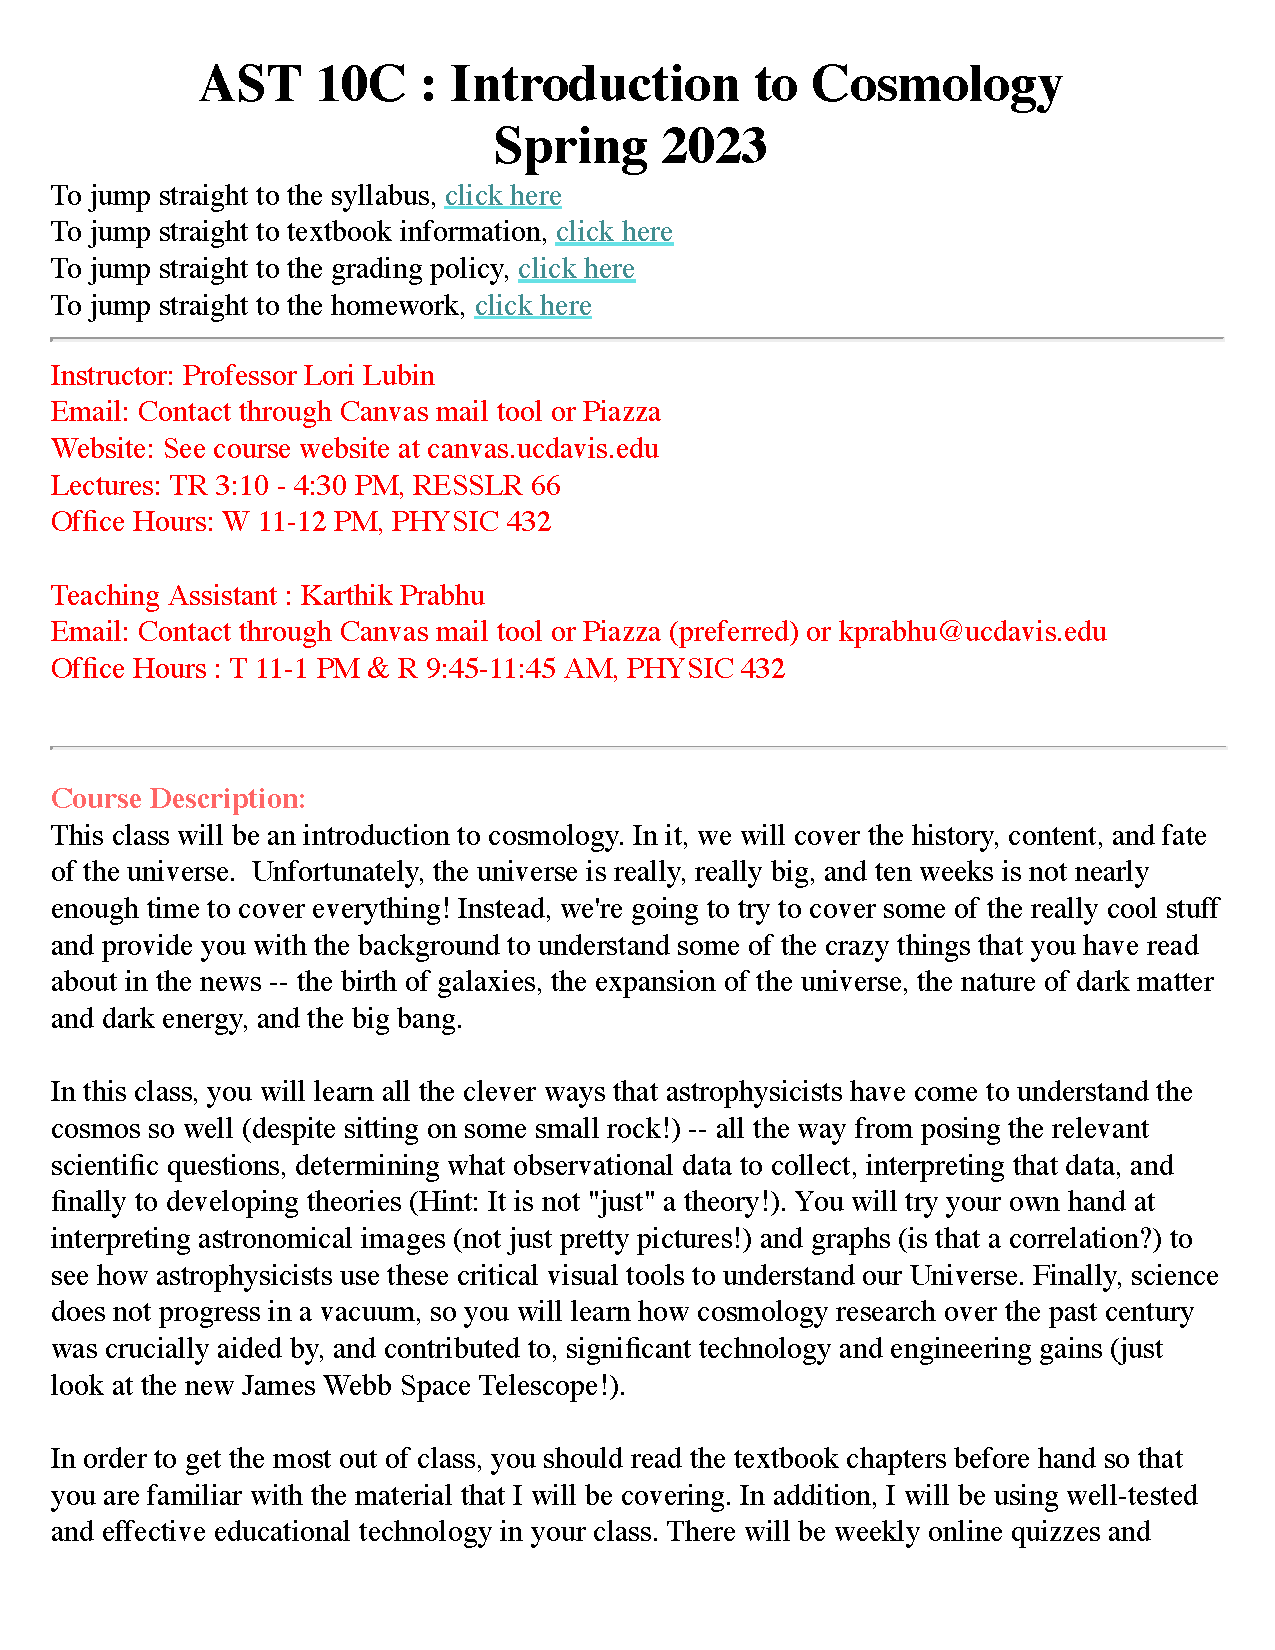
\includepdf[pages=-]{10c/syllabus.pdf}  


\end{document}
